\documentclass[12pt,a4paper]{report}

% --- CẤU HÌNH PHÔNG CHỮ & NGÔN NGỮ ---
\usepackage{fontspec}
\setmainfont{Times New Roman} 

% --- CÁC GÓI LỆNH CẦN THIẾT ---
\usepackage{amsmath}
\usepackage{amsfonts}
\usepackage{amssymb}
\usepackage{graphicx}
\usepackage{array}
\usepackage{hyperref}
\usepackage{geometry}
\usepackage{tikz}

% --- CẤU HÌNH TIÊU ĐỀ CHƯƠNG (Bỏ chữ Chapter, định dạng "1. TÊN CHƯƠNG") ---
\usepackage{titlesec}
\titleformat{\chapter}[hang]{\normalfont\LARGE\bfseries}{\thechapter.}{0.5em}{}
\titlespacing*{\chapter}{0pt}{-10pt}{20pt}
\setcounter{secnumdepth}{4} % Hiển thị số mục đến cấp 4 (Heading 4)

% --- VIỆT HÓA CÁC TỪ KHÓA MẶC ĐỊNH ---
\renewcommand{\contentsname}{MỤC LỤC}
\renewcommand{\listfigurename}{DANH MỤC HÌNH VẼ}
\renewcommand{\listtablename}{DANH MỤC BẢNG BIỂU}
\renewcommand{\bibname}{TÀI LIỆU THAM KHẢO}
\renewcommand{\figurename}{Hình}
\renewcommand{\tablename}{Bảng}

% Cấu hình lề trang theo chuẩn
\geometry{left=3cm, right=2cm, top=2.5cm, bottom=2.5cm}

\begin{document}

% ==================== TRANG BÌA ====================
\begin{titlepage}
    \begin{tikzpicture}[remember picture, overlay]
        \draw[line width=1.5pt] 
            ([xshift=3cm,yshift=-2.5cm]current page.north west) 
            rectangle 
            ([xshift=-2cm,yshift=2.5cm]current page.south east);
    \end{tikzpicture}

    \begin{center}
        \vspace*{0.5cm}
        \large \textbf{ĐẠI HỌC BÁCH KHOA HÀ NỘI} \\
        \large \textbf{TRƯỜNG ĐIỆN - ĐIỆN TỬ}
        
        \vspace{2.5cm}
        \Huge \textbf{BÁO CÁO}
        
        \vspace{2cm}
        \large \textbf{ĐỒ ÁN CHUYÊN NGÀNH II}
        
        \vspace{1.0cm}
        {\Large \textbf{Nghiên cứu, thiết kế và chế tạo hệ thống phân tích đáp ứng tần số và đánh giá chất lượng mạch khuếch đại}}
        
        \vspace{2.5cm}
        \begin{table}[h]
            \centering
            \large
            \renewcommand{\arraystretch}{1.3}
            \begin{tabular}{ll}
                \textbf{Sinh viên thực hiện:} & Nguyễn Duy Anh – 20241652E \\
                                             & Nguyễn Văn Dương – 20241713E \\[0.5cm]
                \textbf{Người hướng dẫn:}     & TS. Đào Việt Hùng
            \end{tabular}
        \end{table}
        
        \vfill
        \large Hà Nội, 4-2026
        \vspace*{0.5cm}
    \end{center}
\end{titlepage}
% ===================================================

% --- MỤC LỤC & CÁC DANH MỤC ---
\pagenumbering{roman}
\tableofcontents
\newpage

\listoffigures
\newpage

\chapter*{DANH MỤC TỪ VIẾT TẮT}
\addcontentsline{toc}{chapter}{DANH MỤC TỪ VIẾT TẮT}
\begin{table}[h]
    \centering
    \renewcommand{\arraystretch}{1.3}
    \begin{tabular}{|p{3cm}|p{5cm}|p{5cm}|}
        \hline
        \textbf{Viết tắt} & \textbf{Dạng đầy đủ} & \textbf{Giải nghĩa} \\
        \hline
        ADC & Analog-to-Digital Converter & Bộ chuyển đổi tương tự sang số \\ \hline
        DAC & Digital-to-Analog Converter & Bộ chuyển đổi số sang tương tự \\ \hline
        DDS & Direct Digital Synthesis & Kỹ thuật tổng hợp tần số trực tiếp \\ \hline
        DSP & Digital Signal Processing & Xử lý tín hiệu số \\ \hline
        DUT & Device Under Test & Thiết bị/Khối mạch cần đo kiểm \\ \hline
        FFT & Fast Fourier Transform & Phép biến đổi Fourier nhanh \\ \hline
        GUI & Graphical User Interface & Giao diện người dùng đồ họa \\ \hline
        MCU & Microcontroller Unit & Khối vi điều khiển \\ \hline
    \end{tabular}
\end{table}
\newpage

% --- NỘI DUNG CHÍNH ---
\pagenumbering{arabic}

\chapter{MỞ ĐẦU}
\section{Lý do chọn đề tài}
Trong kỹ thuật điện tử, việc phân tích đặc tính đáp ứng tần số của mạch khuếch đại là vô cùng quan trọng. Khả năng đánh giá chính xác các tham số phân tích như hệ số khuếch đại thế (Gain) và độ lệch pha (Phase Shift) giúp cho các kĩ sư có cái nhìn trực quan về thiết kế mạch in hiện có. Tuy nhiên, các thiết bị Signal Analyzer chuyên dụng hiện trường thường có mức giá khá cao và đồ sộ. Do đó, đề tài "\textit{Nghiên cứu, thiết kế và chế tạo hệ thống phân tích đáp ứng tần số và đánh giá chất lượng mạch khuếch đại}" được nhóm đặt ra nhằm hướng tới việc nắm vững kỹ thuật, phát triển được một công cụ đo lường linh hoạt kết hợp giữa vi điều khiển nhúng với phần mềm tính toán. 

\section{Mục tiêu nghiên cứu}
Báo cáo này tập trung vào các mục tiêu thiết kế ban đầu sau:
\begin{itemize}
    \item Đề xuất kiến trúc phần cứng tích hợp vi điều khiển hiệu năng cao, trang bị bộ chuyển đổi tương tự - số (ADC) tin cậy nhằm xử lý khối lượng lớn dữ liệu.
    \item Ứng dụng dải chuyển đổi DAC tĩnh trong vi điều khiển để tạo sóng kích thích. Thiết kế mạch giao tiếp Analog Front-End chuẩn mực sử dụng mạng phân áp tự động (Auto-Ranging) kết hợp dịch mức điện áp (DC Bias) nhằm tối ưu hóa sai số lượng tử của bộ ADC.
    \item Phát triển phần mềm giao diện máy tính trực quan, hỗ trợ tính toán độ lệch pha, hệ số khuếch đại (Gain), biểu diễn đồ thị Bode và thực hiện phân tích phổ FFT dựa trên dữ liệu lấy mẫu.
\end{itemize}

\chapter{TỔNG QUAN VÀ KIẾN TRÚC HỆ THỐNG}
\section{Kiến trúc tổng thể của hệ thống Analyzer}
Dựa trên yêu cầu của thực tiễn đo tín hiệu, kiến trúc hệ thống đề xuất bao gồm 4 khối chức năng chính yếu sau đây:
\begin{itemize}
    \item \textbf{Khối phát tín hiệu (TX):} Khai thác bộ DAC 12-bit nội bộ của STM32 kết hợp mạch lọc thông thấp (Reconstruction Filter) và mạch khuếch đại đệm nhằm loại bỏ hiện tượng răng cưa (Aliasing), cung cấp tín hiệu kích thích dạng hình sin có độ tuyến tính cao.
    \item \textbf{Khối ghép nối và kiểm chuẩn (DUT):} Vị trí ghép nối điện trở đầu vào và đầu ra của mạch khuếch đại cần đo lường.
    \item \textbf{Khối thu tín hiệu (RX - Data Acquisition):} Triển khai cấu trúc tự động điều chỉnh thang đo (Auto-Ranging PGA) sử dụng IC chuyển mạch tương tự (Analog Switch) và mạng điện trở. Cơ cấu này chuẩn hóa đa dạng biên độ tín hiệu đầu vào về dải điện áp $0.3\text{V} - 3.0\text{V}$, đồng thời tích cực bảo vệ ngõ vào vi điều khiển bằng diode kẹp áp (Clamping diode) nhằm ngăn chặn quá áp đột biến.
    \item \textbf{Khối xử lý trung tâm (MCU):} Chịu trách nhiệm điều phối luồng dữ liệu, thực thi cơ cấu quét dải tần số liên tục, tổng hợp chuỗi mẫu qua bộ ADC nội và đồng bộ gói dữ liệu về giao diện máy tính cục bộ.
\end{itemize}

\section{Nghiên cứu hạ tầng ADC / DAC}
Việc lựa chọn sử dụng phần cứng trung gian ADC và DAC bắt buộc độ nhiễu loạn cực thấp. 
Đối với \textbf{bộ thu ADC}, hệ thống đòi hỏi một cơ cấu lấy mẫu (Sampling) đủ tốc lớn để thỏa mãn định lý Nyquist cũng như bảo toàn biên dạng phần tử tần số cao mà không xảy ra méo mó, biến dạng khi chuyển qua digital.

\chapter{THIẾT KẾ PHẦN CỨNG MẠCH ĐO}
\section{Lựa chọn linh kiện chủ chốt}
Với mục đích đáp ứng chu trình tốc độ cao trong xử lý tín hiệu thực, nhóm nghiên cứu đã tra cứu kĩ lưỡng và đưa ra lựa chọn các thành tố phần cứng trọng điểm:
\begin{itemize}
    \item \textbf{Vi điều khiển trung tâm (STM32F407VET6):} Việc sử dụng vi điều khiển STM32F407 cung cấp hiệu suất vượt trội bản mẫu thông thường thông qua kiến trúc ADC lấy mẫu đan xen (Triple Interleaved Mode). Chế độ này đẩy tần số lấy mẫu cực đại lên không gian 7.2 MSPS, đảm bảo tái tạo chính xác trạng thái tín hiệu tại điều kiện tần số thiết kế là 500kHz theo chuẩn Nyquist.
    \item \textbf{Cấu trúc Analog Front-End (AFE) mở rộng:} Phương pháp sử dụng phối hợp DAC 12-bit tích hợp sẵn cùng mạch lọc khôi phục tín hiệu (Reconstruction Filter) hỗ trợ loại trừ sai số tần số cao. Giải pháp này cải thiện độ ổn định và giảm thiểu tính phân mảnh của board mạch in (PCB) so với kiến trúc vi sai mô-đun SPI.
    \item \textbf{Khối bảo vệ đầu vào và mạch dịch mức tuyến tính:} Tín hiệu tiếp nhận từ đối tượng đo lường được khống chế biên độ điện thế, theo sau là khối điều khiển Auto-ranging. Bằng sự thiết lập cố định cấu hình của khối Op-Amp hoạt động tạo dịch mức không đổi +1.65V DC, tín hiệu dao động được đối chiếu ổn định trong thiết kế cực hạn $0.3\text{V} - 3.0\text{V}$, tối ưu thông số sai mức lượng tử trên toàn đồ thị đo thực nghiệm.
\end{itemize}

\section{Cấu trúc sơ đồ nguyên lý phần cứng}
Thiết kế sơ đồ nguyên lý cơ sở bao quát trọn bộ cả hệ khối phát và khối thu...

\textit{--- SẼ BỔ SUNG HÌNH ẢNH SCHEMATIC SAU KHI VẼ XONG TRONG GIAI ĐOẠN TỚI ---}


\chapter{THIẾT KẾ PHẦN MỀM GIAO DIỆN (SOFTWARE \& DSP)}
Bên cạnh phần lý thuyết linh kiện, giao diện lập trình điều khiển trên Desktop PC đóng vai trò cốt lõi trong việc trình bày trực quan và thực thi các thuật toán phân tích chuyên sâu.
\section{Thiết kế Kiến trúc Giao diện UI/UX}
Nền tảng phần mềm đã được cấu trúc hoàn chỉnh sử dụng thư viện PyQt6 và pyqtgraph bằng Python. Kiến trúc phần mềm tách biệt phân khu quản trị thông minh, cho phép thu gọn thành 2 chế độ (Mode) đo chính:
\begin{itemize}
    \item \textbf{Chế độ Single Tone / Passive Oscilloscope:} Nhận dữ liệu thu trực tiếp theo time-domain thời gian thực, đáp ứng khảo sát dạng sóng hiện thuần.
    \item \textbf{Chế độ Network Analyzer (Bode Sweep):} Thực thi thuật toán Quét dải tần tự động, đưa thông số phản hồi về thành ma trận tính toán Bode (Đồ thị Magnitude/Phase).
\end{itemize}

\begin{figure}[htbp]
    \centering
    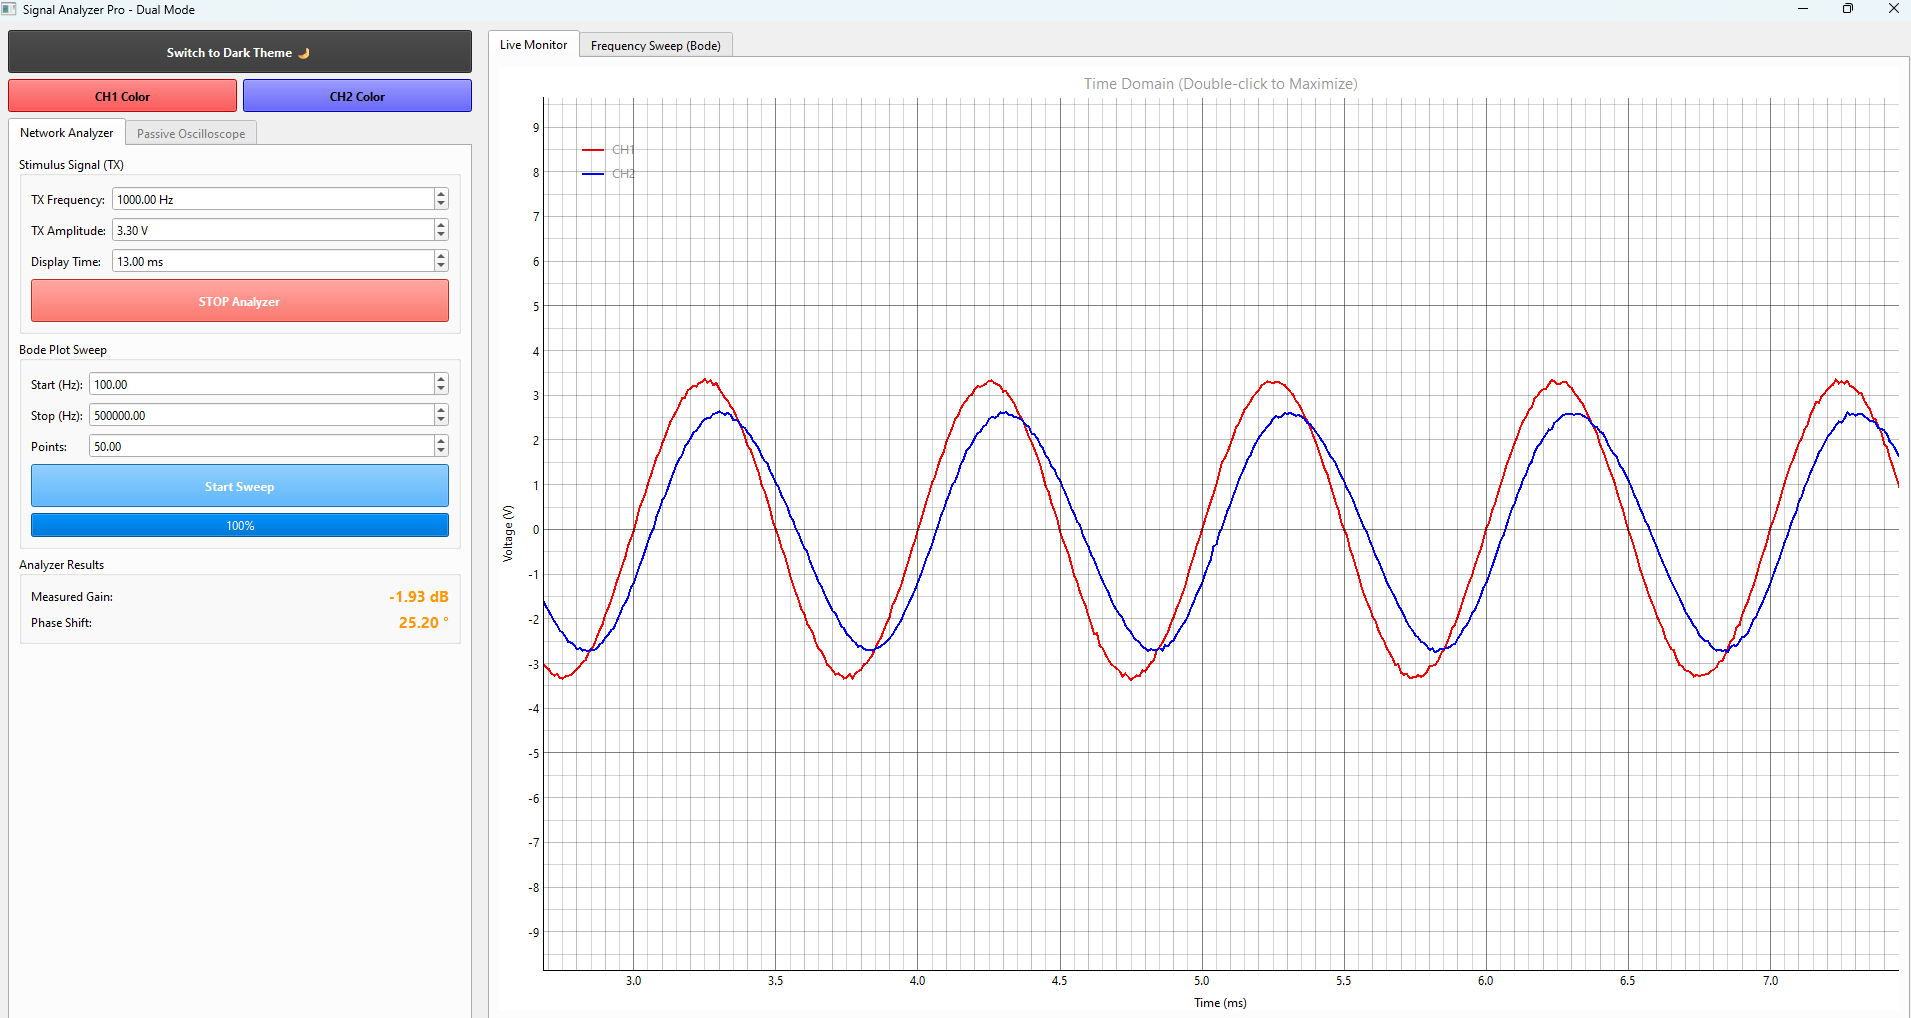
\includegraphics[width=0.9\textwidth]{images/app_desktop1.png}
    \caption{Giao diện chính - Chế độ Trực quan dạng sóng và Phân tích phổ}
    \label{fig:app_desktop1}
\end{figure}

\begin{figure}[htbp]
    \centering
    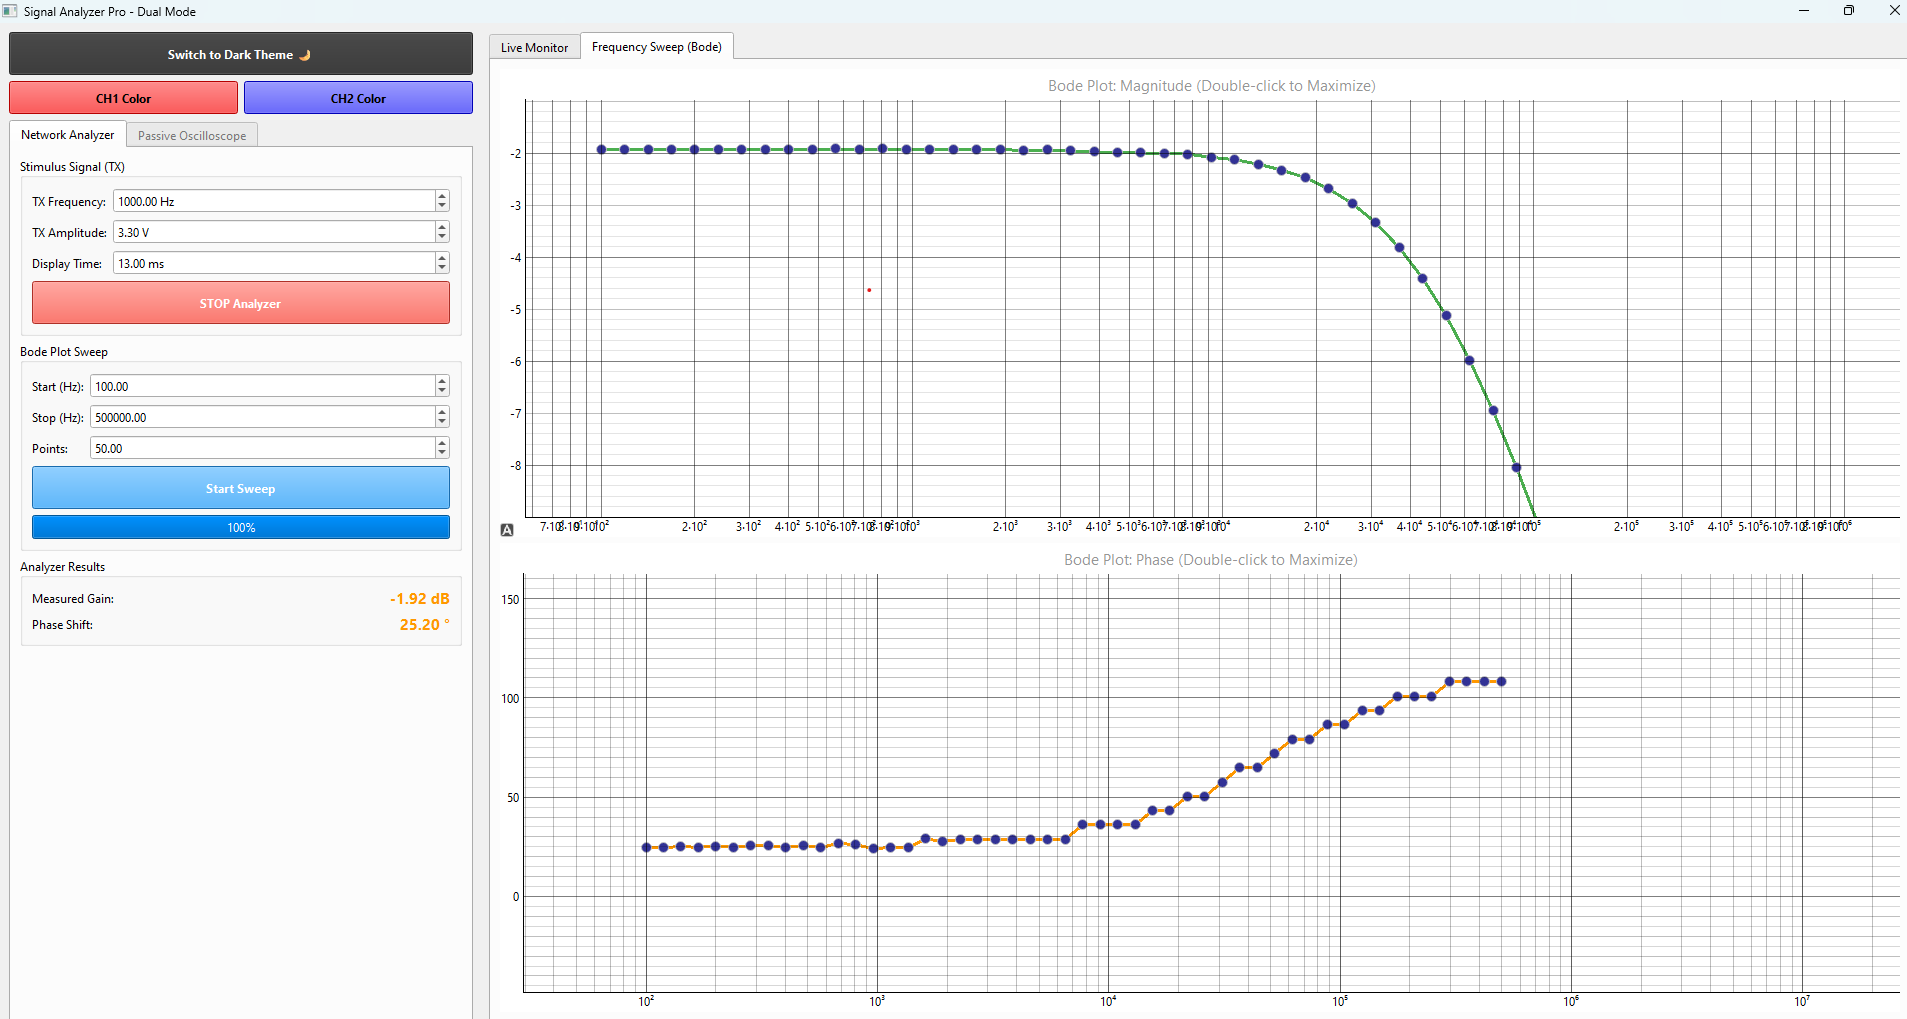
\includegraphics[width=0.9\textwidth]{images/app_desktop2.png}
    \caption{Giao diện chính - Chế độ Quét dải tần và Đồ thị Bode}
    \label{fig:app_desktop2}
\end{figure}

\section{Xây dựng bộ DSP Core xử lý tín hiệu}
Toàn bộ thuật toán lõi đã được xây dựng và mô phỏng xác thực bằng dữ liệu hệ đa phân kì tự sinh. Các thuật toán định danh bao gồm:
\subsection{Thuật toán tính Hệ số khuếch đại (Gain Calculation)}
Để hạn chế sai số quá lố (Outlier) sinh ra bởi nhiễu dạng Gauss trên đỉnh sóng (Peak), thuật toán được thiết kế chuyên sâu dùng thông số kỹ thuật RMS (Root Mean Square - Căn quân phương) làm quy chuẩn. Phương thức nội suy Gain dB giúp cho đường đo Bode trở nên cực mượt ngay cả khi tỉ lệ nhiễu vượt 2\%. 

\subsection{Thuật toán Tương quan chéo đo Phase (Cross-Correlation)}
Dự án thay thế phương pháp "Tìm điểm cắt gốc không" (Zero-crossing detector) truyền thống, sử dụng phép đối sánh tích chập dịch vòng theo "Tương quan chéo" thông qua hàm toán học ma trận của SciPy. Đặc trưng lớn của phương pháp này là loại bỏ hoàn toàn các trường hợp lỗi đo pha ở tần số nhiễu nhỏ, luôn tìm chính xác tỉ lệ trễ tương ứng bằng chỉ số đỉnh độ tương quan sóng cao nhất.

% --- TÀI LIỆU THAM KHẢO ---
\addcontentsline{toc}{chapter}{TÀI LIỆU THAM KHẢO}
\begin{thebibliography}{99}
    \bibitem{1} STMicroelectronics, \textit{STM32F407xx Datasheet - ARM Cortex-M4 32b MCU+FPU}, 2021.
    \bibitem{2} Analog Devices, \textit{AD8307 Low Cost, DC to 500 MHz, 92 dB Logarithmic Amplifier Datasheet}, 2020.
    \bibitem{3} Scipy Contributors, \textit{SciPy Documentation v1.11}, 2023. [Online]. Available: https://docs.scipy.org/doc/scipy/
\end{thebibliography}

\end{document}
